In questo capitolo si vuole verificare la l'efficienza della soluzione implementata. A tal proposito si andranno ad eseguire diversi test per osservare il comportamento assunto dal sistema. Questa analisi permette di comprendere quali siano i punti critici del sistema e fornisce delle informazioni utili per capire in futuro dove andare a effettuare modifiche per ottenere un miglioramento delle \emph{performance}.

Il capitolo si apre con una sezione dedicata allo studio del modello di comportamento del sistema e alla descrizione delle condizioni nei quali sono stati eseguiti i test. Nella sezione successiva verranno svolti diversi test per comprendere quanto tempo il sistema impiega a evadere le richieste e quale sia l'incidenza dei componenti rispetto al tempo totale. Di seguito verrà analizzato il sistema in condizioni d'uso più simili alla realtà, dove diversi utenti interagiscono col sistema e molte richieste devono essere evase nel minor tempo possibile. Si vuole analizzare quale sia il punto di saturazione del sistema e verificare se l'aumento delle caratteristiche della macchina permetta di ottenere dei miglioramenti. Infine viene studiato il comportamento della \emph{mobile app} in diverse condizioni di rete, per capire se l'utente può utilizzare senza problemi l'\emph{app} anche in condizioni nelle quali il collegamento non sia di qualità eccellente.

\section{Sistema di test e modello di simulazione\label{sec:sistema-e-modello}}

In questa sezione si vuole fornire una panoramica del sistema utilizzato e la metodologia seguita per effettuare i test.

Forniamo di seguito alcune definizioni che saranno utili per comprendere i test effettuati:

\begin{itemize}
	\item \textbf{Service Time}
	\upe il tempo che il sistema impiega a completare una richiesta. Tiene conto esclusivamente del tempo impiegato per le elaborazioni, non considerando eventuali ritardi dovuti dal canale di trasmissione o il tempo passato in coda. Viene misurato in secondi
	\item \textbf{Response Time}
	Rappresenta il tempo totale che il sistema impiega a completare una richiesta, compreso il tempo nel quale rimane in coda in attesa che un'istanza si liberi. Viene misurato in secondi
	\item \textbf{Arrival Rate ($ \lambda $)}
	Rappresenta la frequenza con la quale le richieste arrivano al sistema. Viene misurata in richieste al secondo
\end{itemize}

In Figura \ref{fig:sistema-coda} viene mostrata una schematizzazione del flusso di una richiesta.

\begin{figure}[ht]
	\centering
	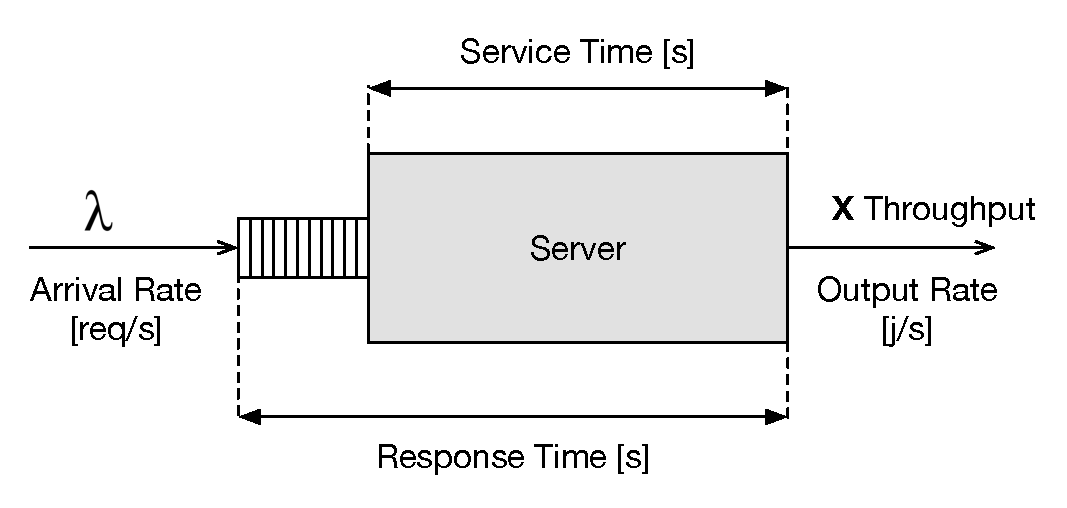
\includegraphics[width=\textwidth]{7-performance/Immagini/sistema_coda.pdf}
	\caption{Sistema a coda singola}\label{fig:sistema-coda}
\end{figure}

Si prosegue con una descrizione del comportamento del sistema. Si è giunti alla conclusione che il sistema in analisi può essere modellato come una coda M/G/1 \cite{sundarapandian2009probability}, in quanto valgono le seguenti considerazioni:

\begin{itemize}
	\item \textbf{M/*/*}
	La probabilità del tempo di arrivo delle richieste al sistema segue una distribuzione \emph{Markoviana}. Le richieste sono indipendenti tra loro e arrivano continuamente a un tasso costante $ \lambda $
	\item \textbf{*/G/*}
	La distribuzione di probabilità dei tempi del servizio non è nota, quindi si assume sia di tipo \emph{Generale}
	\item \textbf{*/*/1}
	Viene utilizzato un singolo processo di Node.js per gestire le richieste in arrivo
\end{itemize}

I test sono stati tutti effettuati su una macchina virtuale. Il motivo di questa decisione è la flessibilità nella scelta dei componenti della macchina, in quanto è possibile variare semplicemente il numero di \emph{core} del processore e la dimensione della RAM. Le caratteristiche del sistema fisico utilizzato vengono elencate nella Tabella \ref{table:performance-pc}.

\begin{table}[ht]
	\caption{Caratteristiche della macchina di test}
	\label{table:performance-pc}
	\centering
	\begin{tabularx}{0.7\textwidth}{lX}
		\toprule
		\thead{Parameter} & \thead{Value} \\ 
		\midrule
		CPU & Intel Core i5-3550 \\
		Cores & 4 \\
		CPU frequency & 3.30GHz \\
		RAM & 8 GB DDR3 \\
		Disk & SSD 60 GB + HDD 1TB \\
		Host OS & Microsoft Windows 10 Pro (on SSD)\\
		VM software & Oracle Virtualbox 5.0 \\ 
		Guest OS & Ubuntu 14.04 (on HDD) \\
		\bottomrule
	\end{tabularx}
\end{table}

Grazie all'utilizzo di una macchina virtuale nei successivi test verranno modificati il numero di \emph{core} della CPU e le dimensioni della RAM. Dove non specificato esplicitamente si assume che la macchina virtuale sia composta da una CPU con 1 \emph{core} e da 1 GB di RAM.

Per limitare il calcolo dei tempi all'interno del confine del sistema, sono state precaricate in \emph{cache} le risposte dei servizi che si andranno ad utilizzare. In questo modo non ci saranno anomalie dovute al tempo necessario per interrogare l'effettivo \emph{server} che gestisce il servizio.

\section{Tempo di risposta a una singola richiesta\label{sec:analisi-service-time}}

In questa sezione si andrà ad analizzare il \emph{Service Time} del sistema. Per evitare che le richieste entrino in coda si attende che la richiesta in corso termini prima di lanciarne un'altra.

Si è innanzitutto effettuata un'analisi per comprendere quali siano i parametri che condizionano il tempo di risposta del servizio. Gli elementi identificati sono:

\begin{itemize}
	\item \textbf{Dimensioni del contesto}
	Il primo passaggio nel \emph{server} è il \emph{parsing} del contesto, quindi si ipotizza che questo punto possa influire sulle prestazioni del sistema. Facendo delle stime su quanto possa essere grande un contesto in condizioni d'uso reali sono stati definiti tre livelli: \emph{i)} piccolo, composto da 2 elementi; \emph{ii)} medio, formato da 5 elementi e \emph{iii)} grande, composto da 8 elementi
	\item \textbf{Numero di servizi}
	Rappresenta il numero di servizi che vengono interrogati per acquisire le informazioni. Queste attività vengono gestite in parallelo però si ritiene comunque che avere più servizi da interrogare possa aumentare i tempi di esecuzione. Perciò sono stati effettuati test con tre livelli, che rappresentano il numero di servizi che vengono invocati
\end{itemize}

Il primo test che si è andati a verificare è come questi due parametri incidono sul \emph{Service Time}. Sono state lanciate 500 richieste per ogni possibile coppia. I risultati possono essere osservati in Figura \ref{fig:service-time-overview}.

\begin{figure}[ht]
	\centering
	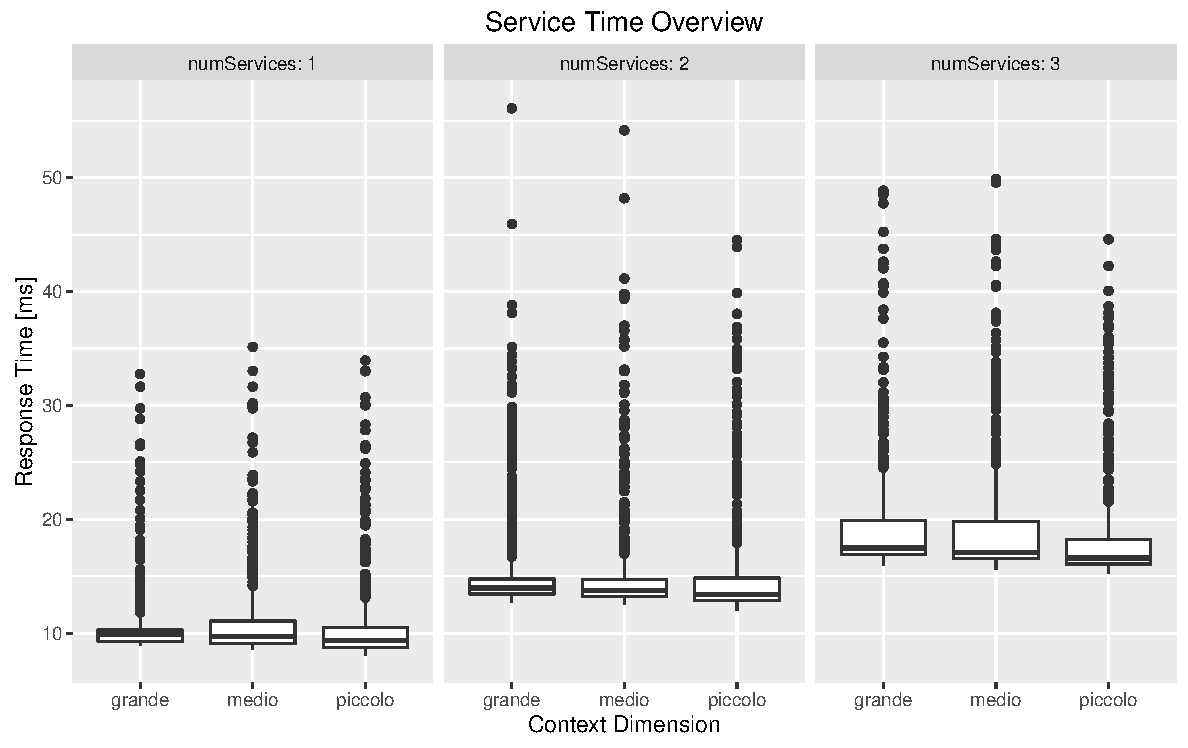
\includegraphics[width=\textwidth]{7-performance/Immagini/service_time_overview.pdf}
	\caption{Analisi del Service Time con differenti configurazioni}\label{fig:service-time-overview}
\end{figure}

Come ci si poteva aspettare, vista la relativa vicinanza tra le tre tipologie di contesto, non ci sono grosse variazioni dovute alla dimensione del contesto, se non un leggero aumento man mano che aumentano le sue dimensioni. Invece si può notare come l'operazione che più incide è il numero di servizi da invocare. In questo caso il divario è più netto, a causa del maggior carico richiesto per completare queste attività.

In Figura \ref{fig:service-time-distribution} viene mostrata la distribuzione dei tempi di risposta con dimensione grande del contesto e tre servizi interrogati.

\begin{figure}[ht]
	\centering
	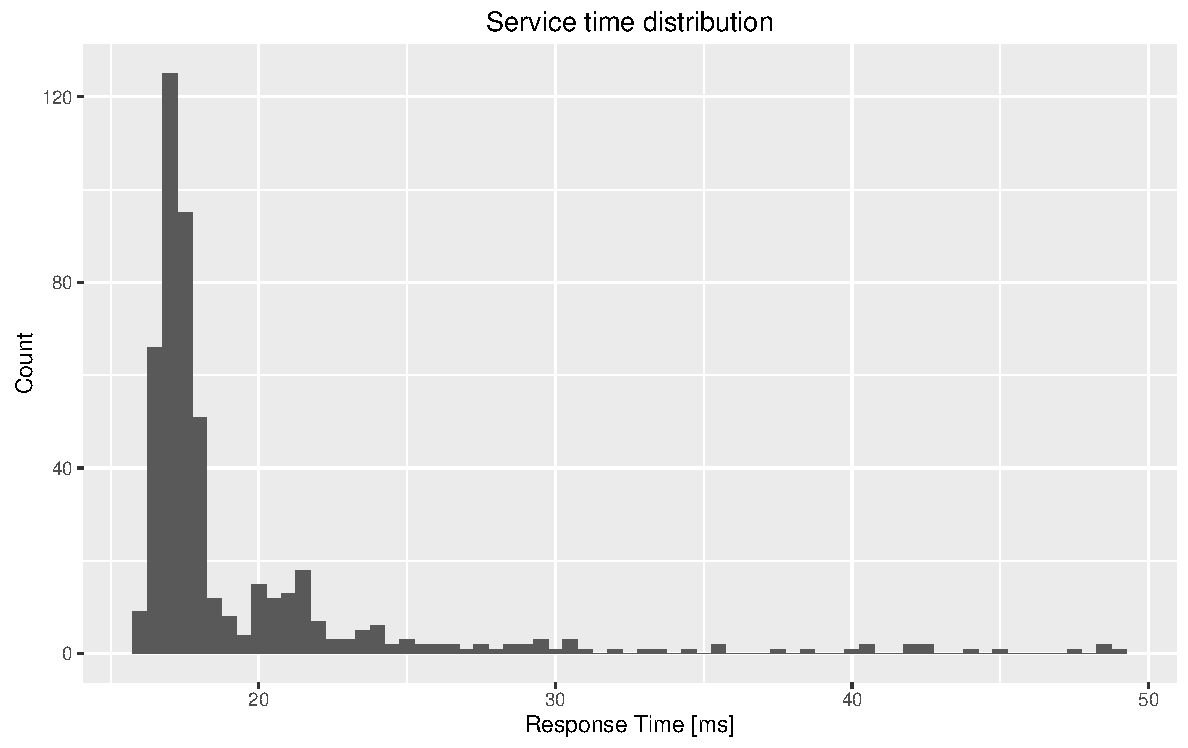
\includegraphics[width=\textwidth]{7-performance/Immagini/service_time_distribution.pdf}
	\caption{Distribuzione del Service Time}\label{fig:service-time-distribution}
\end{figure}

Risulta un tempio medio di esecuzione pari a 19,5 ms mentre il caso peggiore è di 48,86 ms. Quest'ultimo valore ci permette di calcolare l'\emph{arrival rate} di saturazione, che rappresenta il limite massimo dopo il quale si verifica un accodamento delle richieste. Questo valore risulta essere pari a 20,46. Verrà verificato nella sezione successiva dove saranno eseguiti test con diversi valori di $ \lambda $.

Un ulteriore test che si è andati a eseguire riguarda l'incidenza dei singoli componenti in una richiesta. La configurazione utilizzata è la medesima del test precedente. \upe stata poi calcolata una media dei tempi raccolti divisi per singolo componente e separati ulteriormente in tre categorie:

\begin{enumerate}
	\item \textbf{Elaboration}
	Rappresenta il tempo speso in elaborazioni
	\item \textbf{Database}
	\upe il tempo speso nell'effettuare le \emph{query} verso il database MongoDB
	\item \textbf{External}
	\upe il tempo necessario per interrogare i servizi. In questo caso rappresenta il tempo necessario per recuperare la risposta da Redis
\end{enumerate}

In questo modo, oltre a osservare l'impatto di ogni componente sul tempo totale, è possibile capire anche quali siano le attività più onerose eseguite dal componente stesso. I risultati di questa analisi vengono mostrati in Figura \ref{fig:component-time}.

\begin{figure}[ht]
	\centering
	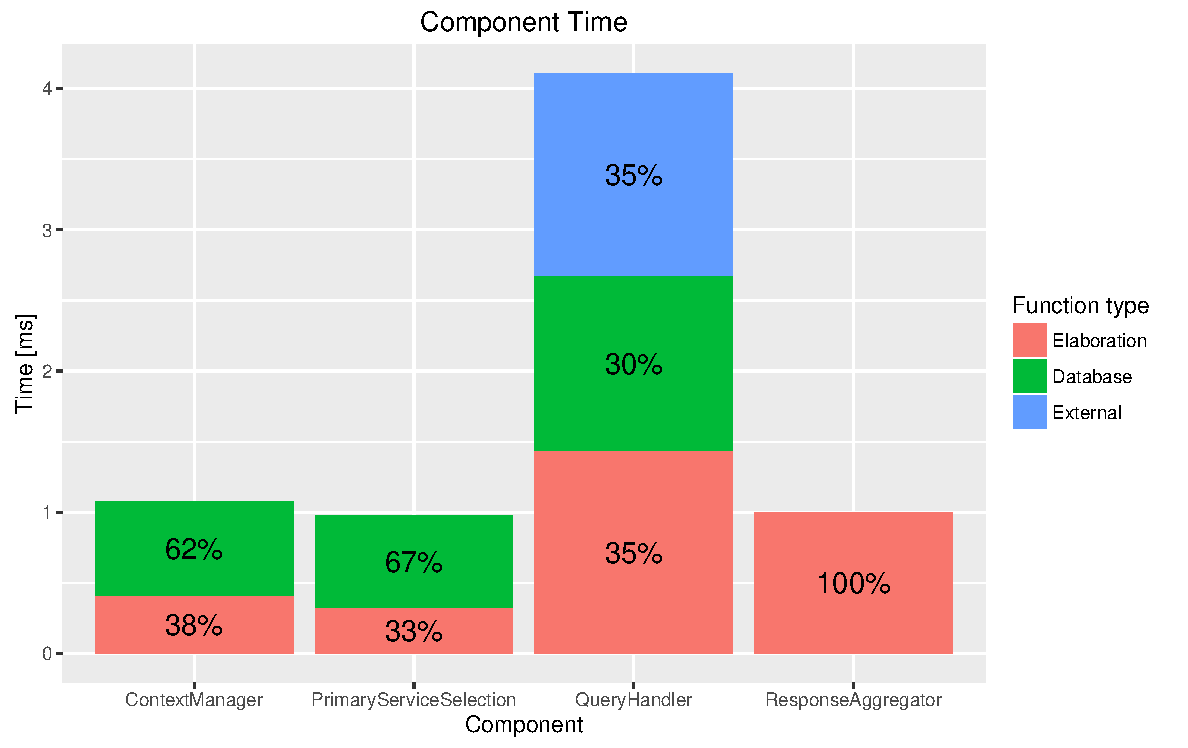
\includegraphics[width=\textwidth]{7-performance/Immagini/component_time.pdf}
	\caption{Analisi del tempo di esecuzione dei componenti}\label{fig:component-time}
\end{figure}

Come ci si poteva aspettare dopo il primo test, il componente che ha un'incidenza maggiore è il \emph{Query Handler}, che si occupa proprio di interrogare i servizi e trasformare le risposte. \upe l'unico componente che esegue tutte e tre le tipologie di attività ed esse sono praticamente equidivise in termini di tempo di esecuzione. Gli altri componenti hanno all'incirca il medesimo impatto sul tempo di esecuzione. Si può osservare che per il \emph{Context Manager} e il \emph{Primary Service Selection} la maggior parte del tempo viene speso nell'interrogare il database. Invece il \emph{Response Aggregator} trascorre tutto il tempo in elaborazioni, in quanto analizza i dati ricevuti dai servizi senza la necessità di interrogare il database.

\section{Tempo di risposta per richieste multiple\label{sec:analisi-response-time}}

In questa sezione si vuole verificare come si comporta il sistema in condizioni d'uso più simili alla realtà. Vengono eseguite richieste multiple che rappresentano le interazioni dei diversi utenti con il sistema. Verrà dunque misurato il \emph{Response Time} di ogni richiesta, in quanto in alcuni casi le richieste saranno accodate prima di essere eseguite. Come esposto nella Sezione \ref{sec:sistema-e-modello} la distribuzione degli arrivi è continua e indipendente, quindi è stata scelta una \emph{distribuzione esponenziale} per determinare i tempi di arrivo delle richieste:

\begin{equation}
	f(x;\lambda) = 
	\begin{cases}
		\lambda e^{-\lambda x} & \text{se } x \ge 0 \\
		0 & \text{se } x < 0
	\end{cases}
\end{equation}

dove $ \lambda $ definisce l'\emph{arrival rate} delle richieste e \emph{x} il tempo tra una richiesta e la successiva.

Si è dunque variato il valore di $ \lambda $ in un intervallo $ [5, 100] $ per osservare il comportamento del sistema all'incrementare del numero di richieste. Si è voluto inoltre andare a osservare se il sistema sia realmente scalabile: a tal scopo è stato ripetuto questo test con diverse configurazioni della macchina virtuale, andando ad aumentare il numero di \emph{core} della CPU e la dimensione della RAM. I risultati vengono mostrati in Figura \ref{fig:exponential-analysis}.

\begin{figure}[ht]
	\centering
	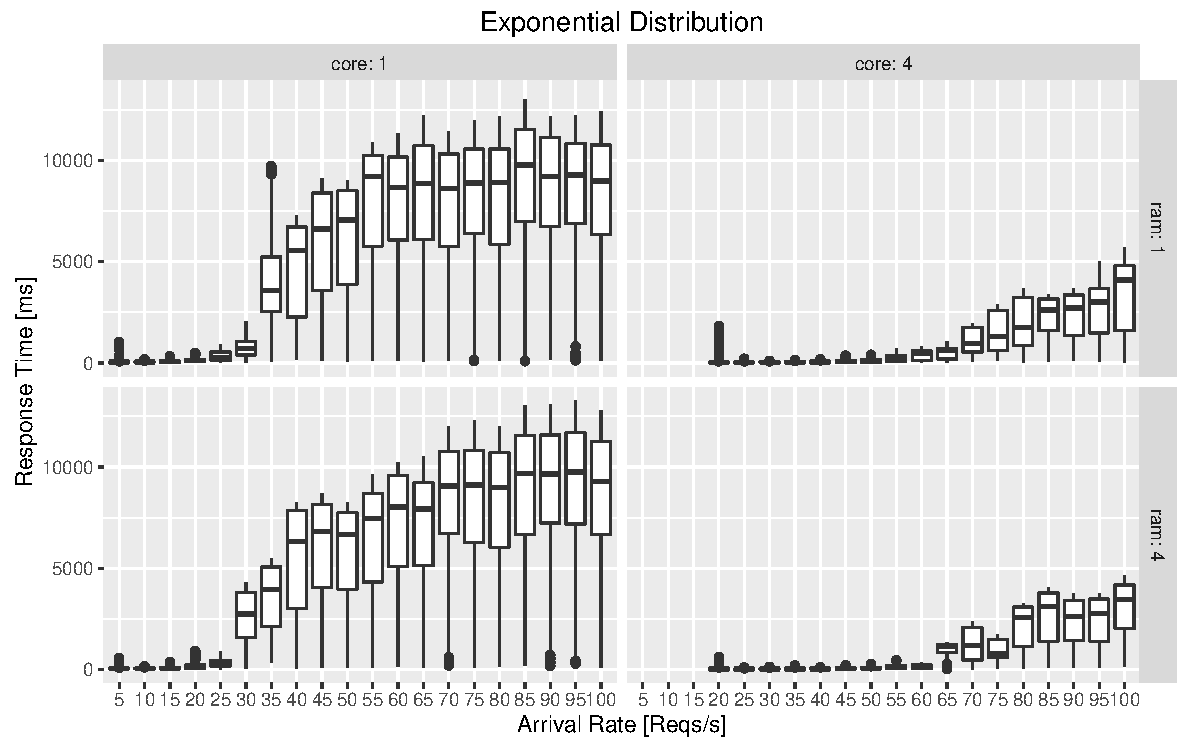
\includegraphics[width=\textwidth]{7-performance/Immagini/exponential_analysis.pdf}
	\caption{Analisi del Response Time con differenti configurazioni}\label{fig:exponential-analysis}
\end{figure}

Come si può notare nel primo quadrante il sistema rimane stabile fino ad un valore di $ \lambda $ pari a 20, dopo di che le richieste incominciano ad essere inserite in coda. Questo valore è congruo con quanto calcolato nella Sezione \ref{sec:analisi-service-time}. Un dato interessante è che il variare delle dimensioni della RAM non presenta evidenti benefici. Questo risultato può essere dovuto alle relative ridotte dimensioni del database, che quindi non necessita di grandi quantitativi di memoria per essere elaborato. In situazioni nelle quali il database assume dimensioni più importanti questo parametro farà sicuramente sentire il suo peso.

Più interessante è il risultato ottenuto impostando la macchina virtuale con 4 \emph{core}. \upe possibile chiaramente notare un grosso miglioramento nella velocità di esecuzione. Nel caso migliore si passa da un $ \lambda $ pari a 20 ad uno pari a 60, ottenendo così una capacità del sistema di evadere il triplo delle richieste senza doverle accodare. Questo miglioramento è dovuto per la maggior parte al database MongoDB, che è l'unico elemento del sistema studiato per sfruttare più \emph{core} del processore. Sia Node.js sia Redis lavorano invece con un solo \emph{thread}: per ottenere migliori performance è necessario mettere in funzione diverse repliche dei processi principali, in modo che le richieste vengano smistate verso il nodo più libero.

\section{Tempo di risposta con condizioni di rete diverse\label{sec:analisi-condizioni-rete}}

Oltre ai test sul carico del \emph{server} sono state effettuate delle valutazioni per quanto riguarda le diverse condizioni di utilizzo dell'applicazione \emph{mobile}. Avendo scelto come caso di studio quello del turismo è sorto spontaneo chiedersi in che modo l'applicazione reagisse in movimento e in diverse condizioni di rete. Per esempio se l'utente si trova a casa propria sotto rete WiFi la velocità di caricamento dei risultati sarà diversa da quella misurata mentre si trova in alta montagna, dove la copertura di rete è spesso minima.

Per valutare se i tempi di attesa rimangano sempre accettabili si è scelto di utilizzare il simulatore iOS e uno strumento aggiuntivo che introduce un ritardo nel caricamento dei dati a seconda delle diverse condizioni di rete specificate. A partire da questo si sono scelte le tre condizioni di rete più significative: WiFi, 3G ed Edge.
All'interno dell'applicazione è stato utilizzato un metodo di test che effettua un numero significativo di richieste verso il \emph{server}. Il test viene effettuato utilizzando 50 richieste una di seguito all'altra, in modo da non peggiorare il tempo di risposta caricando eccessivamente il \emph{server}. La \emph{query} utilizzata è quella di tipo ristoranti, continuamente ripetuta.

Nella Tabella \ref{table:connections-data-test} sono mostrati i parametri delle condizioni di simulazione, dove l'ADSL indica la connessione internet utilizzata dal computer e gli altri parametri sono quelli utilizzati nello strumento di modifica delle condizioni di rete. Come si può notare le aspettative di tempi di risposta in ordine crescente sono WiFi, 3G ed Edge.

\begin{table}[ht]
	\caption{Analisi velocità delle connessioni}
	\label{table:connections-data-test}
	\begin{tabularx}{\textwidth}{CCCCC}
		\toprule
		\thead{Connection Type} & \thead{Download Speed} & \thead{Upload Speed} & \thead{Total Delay}  \\
		\midrule
			ADSL & 7 Mb/s & 340 Kb/s &\\ 
			\hline
			Edge & 240 Kb/s & 200 Kb/s & 840 ms \\ 
			3G  & 780 Kb/s & 330 Kb/s & 200 ms \\
			WiFi  & 40 Mb/s & 33 Mb/s & 2 ms \\
		\bottomrule
	\end{tabularx}
\end{table}

Nella Figura \ref{fig:network-time-analysis} sono mostrati i risultati medi per ogni condizione di rete. Come ci si poteva aspettare i tempi di risposta più bassi sono dati dalla connessione WiFi, seguiti dal 3G e infine dalla Edge. La differenza tra WiFi e 3G è molto meno marcata, soprattutto perché per provare il tempo risposta è stata utilizzata una connessione a monte non molto performante, mentre per quanto riguarda la connessione Edge c'è molta più differenza, come del resto era prevedibile dalle condizioni di simulazione. In qualunque caso, con l'utilizzo della paginazione per un caricamento scaglionato dei dati e le loro ridotte dimensioni, anche i tempi di risposta in condizioni sfavorevoli non sono così elevati, consentendo all'utente in qualsiasi caso una soddisfacente esperienza d'uso.

\begin{figure}[ht]
	\centering
	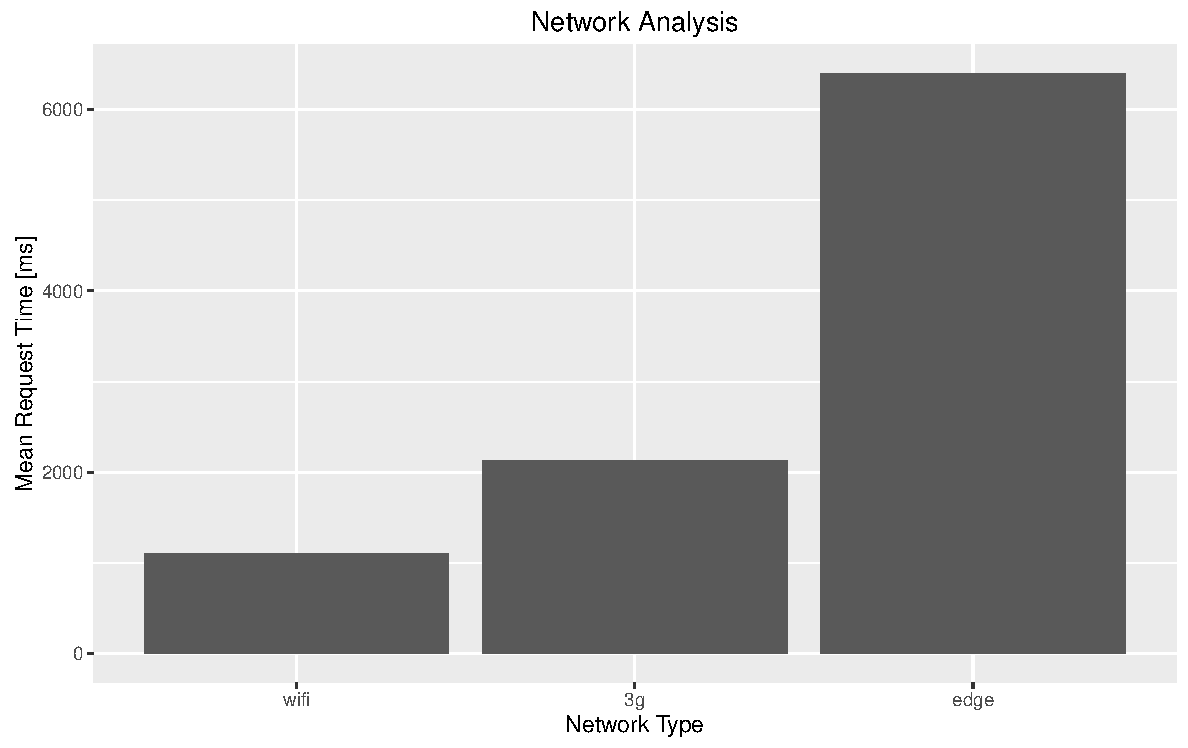
\includegraphics[width=\textwidth]{7-performance/Immagini/network_time_analysis.pdf}
	\caption{Analisi dei tempi di risposta con reti diverse}\label{fig:network-time-analysis}
\end{figure}